\documentclass{ctexrep}
\usepackage{graphicx}


\begin{document}

\title{GNU C Compiler \& Makefile}
\author{ }
\maketitle


%=====   section 1  =====
\section{编译过程简介}

\begin{figure}[hbt]
	\centering
    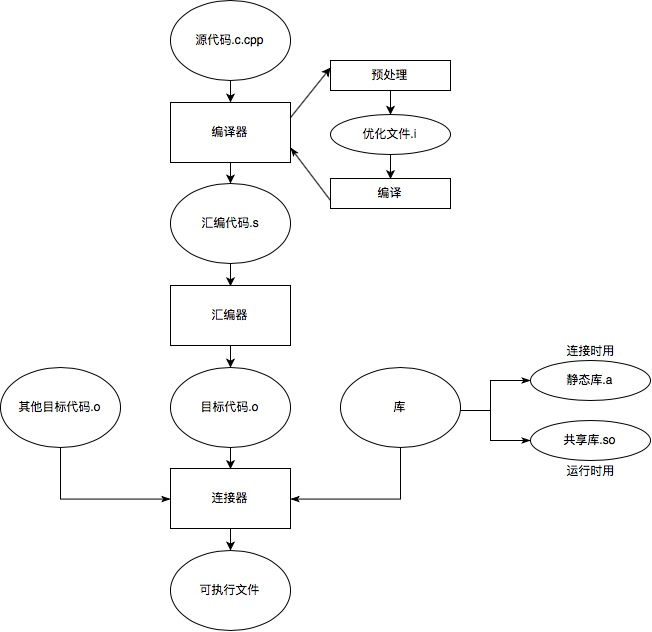
\includegraphics[width=\linewidth]{compiler.jpg}
    \caption{编译基本过程}
    \label{编译过程框图}
\end{figure}

%=====   section 2  =====
\section{GNU C Compiler(gcc/g++)}
命令格式:\par
    \textbf{gcc/g++ [command] [filename] [command] [filename]}

其中command可以是:
\begin{itemize}
    \item [-]c (compiler):编译,可以将源代码编译成目标代码,或将汇编代码编译到目标代码.
    \item [-]o (object file):指示目标文件.
    \item [-]E:只生成预处理结果
    \item [-]S:只生成汇编代码
    \item [-]Wall:显示警告
    \item [-]I:指示include文件
    \item [-]L:指示lib文件
    \item [-]l:指示依赖项.
\end{itemize}


%=====   section 3  =====
\section{关于Makefile}

文件格式:\par
	\textbf{执行文件: 目标文件1.o 目标文件2.o \# 指示依赖关系}\par
	\textbf{\qquad tab\footnote{'tab'表示这里需要一个制表符} gcc 目标文件1.o 目标文件2.o -o 执行文件 \# 指示具体操作}\par
	\textbf{目标文件1.o : 源文件1.c}\par
    \textbf{\qquad tab gcc -c 源文件1.c -o 目标文件1.o}\par
	\textbf{... \# 其他目标文件}\par
		\qquad...\par
	\textbf{clean:}\par
	\textbf{\qquad rm -rf *.o 执行文件 \# 删除目标文件(.o) 删除执行文件}\par
	\textbf{\qquad ... \# 删除其他中间文件}\par

\vspace{6pt}
有用的函数:
\begin{enumerate}
    \item wildcard:通配符:SOURCE = \$(wildcard *.c *.cpp),其中SOURCE为所有.c.cpp文件的列表.*为通配符.参数之间用空格隔开.
    \item patsubst:替换\\
1.OBJECTS = \$(patsubst \%.c,\%.o,\$(SOURCE)),将所有.c文件换成.o文件.\%用于匹配字符,\%.c代表所有.c结尾的文件.\\
2.OBJECTS = \$(patsubst \%.c,\%.o,\$(patsubst,\%.cpp,\%.o,\$(SOURCE))),替换所有.c.cpp文件.\\
\end{enumerate}


\vspace{6pt}
特殊符号:
\begin{enumerate}
    \item \%: ''在依赖文件.o:和源文件.c''处,可用\%.o:\%.c代替.
    \item \$@表示目标文件集。
    \item \$<依赖目标中的第一个目标名字。如果依赖目标是以模式(即"\%")定义的,那么"\$<"将是符合模式的一系列的文件集。注意,其是一个一个取出来。所有比目标新的依赖目标的集合。以空格分隔。
    \item \$\^所有的依赖目标的集合。以空格分隔。如果在依赖目标中有多个重复的,那个这个变量会去除重复的依赖目标,只保留一份。
\end{enumerate}



\end{document}
